
\section{Narzędzia topologiczne}
\label{sec:topmeth}

W tej części wprowadzimy główne narzędzia topologiczne wykorzystane w tej pracy.
Kluczowym pojęciem będzie pojęcie {\em relacji nakrywającej } i {\em h-setu} \cite{ZGi}
%In this section we present  main topological tools used in this
%paper. The crucial notion is that of {\em  covering relation}
%\cite{ZGi}.

\subsection{h-sets}



\begin{definition} \cite{ZGi}
\label{def:covrel} h-set, $N$, jest to obiekt składający się z czterech
częsci
%is the  object consisting of the
%following data
\begin{itemize}
 \item $|N|$  - zwarty podzbiór ${\mathbb R}^n$, będziemy nazywać go suportem h-setu $N$ %- a compact subset of ${\mathbb R}^n$
 \item $u(N),s(N) \in \{0,1,2,\dots\}$, takie, że $u(N) + s(N) = n$ % such that $u(N)+s(N)=n$
 \item homeomorfizmu $c_N:{\mathbb R}^n \to   
   {\mathbb R}^n={\mathbb R}^{u(N)} \times {\mathbb R}^{s(N)}$,
    % a homeomorphism $c_N:{\mathbb R}^n \to
	 takiego że zachodzi : %    such that
      \begin{displaymath}
        c_N(|N|)=\overline{B_{u(N)}}(0,1) \times
        \overline{B_{s(N)}}(0,1).
      \end{displaymath}
\end{itemize}
Definiujemy następująco : 
\begin{eqnarray*}
  N_c=\overline{B_{u(N)}}(0,1) \times \overline{B_{s(N)}}(0,1), \\
   N_c^-=\partial \overline{ B_{u(N)}}(0,1) \times
\overline{B_{s(N)}}(0,1) \\
N_c^+=\overline{B_{u(N)}}(0,1) \times
\partial \overline{B_{s(N)}}(0,1) \\
  N^-=c_N^{-1}(N_c^-) , \quad N^+=c_N^{-1}(N_c^+)
\end{eqnarray*}
\end{definition}

Reasumując {\em h-set }  $N$ jest iloczynem kartezjańskim dwóch domkniętych kul w jakimś
układzie współrzędnych. Liczby $u(N)$ i $s(N)$ to wymiary odpowiednio nominalnie niestabilnego
i stabilnego kierunku. Indeks $c$ odpowiada nowemu układowi współrzędnych zadanego poprzez homeomorfizm
$c_N$. Zauważmy, że jeżeli $u(N) = 0$ wtedy $N^-=\emptyset$ a jeżeli $s(N)=0$, wtedy $N^+=\emptyset$.
Jeżeli to będzie jasne z kontekstu by nie zaciemniać przekazu będziemy opuszczać pionowe kreski
przy oznaczeniu suportu h-setu $N$. Czyli $N$ będzie oznaczało zarówno h-set jaki i jego suport.

\subsection{Relacje nakrywające}
\begin{definition} \cite{ZGi}
\label{def:covw} 
Załóżmy że $N,M$ są {\em h-setami}, takimi że: $u(N)=u(M)=u > 0$ i $(s(N)=S(M)=s$.
Niech $f:N \to {\mathbb R}^n$ będzie odwzorowaniem ciągłym. 
Definiujemy $f_c = c_M \circ f \circ c_N^{-1}: N_c \to {\mathbb R}^u \times {\mathbb R}^s $.
Niech $w$ będzie niezerową liczbą całkowitą. 
Mówimy, że 
\begin{displaymath}
  N\cover{f,w} M
\end{displaymath}
($N$ $f$-nakrywa $M$ w stopniu $w$) wtedy i tylko wtedy jeżeli zachodzą następujące warunki
\begin{description}
\item[1] 
   Istnieje ciągła homotopia $h:[0,1]\times N_c \to {\mathbb R}^u \times {\mathbb R}^s$ spełniająca następujące
   warunki
   \begin{eqnarray}
      h_0&=&f_c,  \label{eq:hc1} \\
      h([0,1],N_c^-) \cap M_c &=& \emptyset ,  \label{eq:hc2} \\
      h([0,1],N_c) \cap M_c^+ &=& \emptyset .\label{eq:hc3}
   \end{eqnarray}
\item[2] 
	Istnieje odwzorowanie $A:{\mathbb R} ^u \to {\mathbb R}^u$ takie że:
   \begin{eqnarray}
    h_1(p,q)&=&(A(p),0), \mbox{ for $p \in \overline{B_u}(0,1)$ and $ q \in
    \overline{B_s}(0,1)$,}\label{eq:hc4}\\
      A(\partial B_u(0,1)) &\subset & {\mathbb R}^u \setminus
      \overline{B_u}(0,1).  \label{eq:mapaway}
   \end{eqnarray}
  %Moreover, we require that
  Co więcej zakładamy że :
\begin{displaymath}
  \deg(A,\overline {B_u}(0,1),0)=w,
\end{displaymath}
\end{description}
\end{definition}

Intuicyjnie nasz definicja mówi, że $N \cover{f} N$ jeżeli $f$ rozciąga $N$ w kierunku
'nominalnie niestabilnym', w taki sposób, że jego rzut na 
'nominalnie niestabilny' kierunek w $M$ pokrywa w topologicznie nietrywialny sposób rzut $M$.
W 'nominalnie stabilnym' kierunku $N$ jest zwężane przez $f$. W rezultacie $N$ jest odwzorowane
poprzez $M$ w kierunku niestabilnym bez dotykania $M^+$. 
Warto zauważyć również że stopień $w$ w relacji nakrywającej zależy jedynie
od $A_{|\partial B_u(0,1)}$


Geometria definicji  \ref{def:covw} przedstawiona jest na 
Rysunku .~\ref{fig:cover}.

\begin{figure}[htbp]
\centerline{
    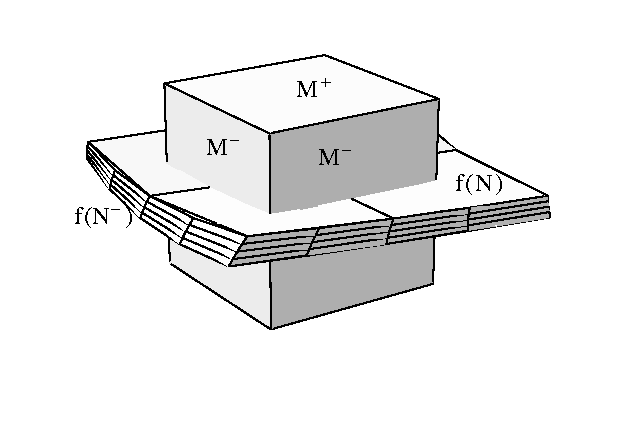
\includegraphics[width=.5\textwidth]{cover.eps}
    }
\caption{Ilustracja relacji nakrywającej $N\cover{f}M$. W przypadku $u(N)=u(M)=2$ and $s(N)=s(M)=1$.\label{fig:cover}}
\end{figure}

\begin{definition}\label{def:horizontalDisk}
Niech $N$ będzie $h-set$em. Niech $ b:\overline{B_{u(N)}}(0,1) \to |N| $
będzie odwzorowanie i zdefiniujmy $b_c = c_N \circ b$. Odwzorowanie b nazywamy dyskiem poziomym w N jeżeli istnieje ciągła homotopia $ h: [0,1] \times \overline{B_{u(N)}}(0,1) \to
N_c $ taka, że :
	
\begin{eqnarray*}
    h_0&=&b_c, \\
    h_1(x)&=&(x,0),\quad \forall x \in \overline{B_{u(N)}(0,1)}\\
    h(t,x)&\in &N^-_c,\quad \forall t \in [0,1] \mbox{ i } x \in \partial B_{u(N)}(0,1)
\end{eqnarray*}
\end{definition}

\begin{definition}\label{def:verticalDisk}
Załóżmy, że $N$ będzie {\em h-setem}. Niech $ b:\overline{B_{s(N)}}(0,1) \to |N| $
będzie odwzorowanie i zdefiniujmy $b_c = c_N \circ b$. Odwzorowanie b nazywamy dyskiem pionowym w N jeżeli istnieje ciągła homotopia $ h: [0,1] \times \overline{B_{s(N)}}(0,1) \to
N_c $ taka, że :
	
\begin{eqnarray*}
    h_0&=&b_c, \\
    h_1(x)&=&(0,x),\quad \forall x \in \overline{B_{s(N)}}(0,1)\\
    h(t,x)&\in &N^+_c,\quad \forall t \in [0,1] \mbox{ i } x \in \partial B_{s(N)}(0,1)
\end{eqnarray*}
\end{definition}

Zauważmy, że dysk poziomy w $N$ może również być dyskiem pionowym w $N$. Przykład :
// tutaj obrazek

\begin{theorem}
	Niech będzie $k \geq 1 $. Załóżmy , że $N_i, i = 0, \dots ,k $ są h-setami
	i dla każdego $ i = 0, \dots ,k $ zachodzi 
	\begin{eqnarray*}
  		N_{i-1} \cover{f_i,w_i} N_i
	\end{eqnarray*}
	Załóżmy, że $b_0$ jest poziomym dyskiem w $N_0$ i $b_e$ jest pionowym dyskiem
	w $ N_k$ 
	Wtedy istnieje punkt $ x \in \inte N_0$, taki  że:
	\begin{eqnarray*}
   	x&=&b_0(t), \quad \mbox{Dla jakiegoś } t \in B_{u(N_0)}(0,1) \\
    f_i \circ f_{i-1} \circ \dots f_1(x) &\in &\inte N_i, \quad i = 1, \dots , k \\
    f_k \circ f_{i-1} \circ \dots f_1(x) &=& b_e(z) ,\quad \mbox{Dla jakiegoś } t \in B_{u(N_0)}
\end{eqnarray*}
\end{theorem}

Rozważmy szczególny przypadek tego twierdzenia. Mianowicie kiedy nasze $h-sety$ leżą na
płaszczyźnie i $u(N_i) = s(N_i) =1 $ dla $ i=0, \dots k $. Wtedy dowód staję się bardzo
prosty i chciałbym go tutaj przytoczyć. Zanim jednak przejde do dowodu tego twierdzenia musze przytoczyć pewien potrzebny lemat.

\begin{lemma}
  Niech $ N $ będzie h-setem takim, że $ u(N) = 1 $ i $ s(N) = 1 $.
  Niech $ h $ będzie dyskiem poziomym w $ N $ a $ g $ dyskiem pionowym w $ N $.
  Wtedy te dwa dyski się przecinają, tzn istnieje takie $ t_g \in [-1,1] $ i $ t_h \in [-1,1] $
  takie, że $ g(t_g) = h(t_h) $
 \end{lemma}
  Dowód:
  \newline
  Niech $ c $ będzie homeomorfizmem z definicji {\em h-setu } $ N $.
  Przecięcia $ h $ i $ g $ jest równoważne przecięciu $ h_c $ i $ g_c $ 
  
  Niech $H_h, H_g $ to będą odpowiednie homotopie z definicji dysków.
  Niech $ \pi_1,\pi_2 $ to będą rzutowania na odpowiednio na pierwszą i drugą współrzędną.	
  Rozważmy funkcje $ f : [-1,1] \times [-1,1] \to \mathbb R^2 $ zdefiniowaną następująco :
  \begin{equation}
    f(t_1,t_2) = h_c(t_1) - g_c(t_2)
  \end{equation}
  Szukanie przecięcia tych dwóch dysków sprowadza się do szukanie zer wyżej wymienionej funckji.
  Jeżeli nasza funckja zeruje się na brzegu kuli na której jest zdefiniowana to znaleźliśmy szukane przecięcie.
  Załóżmy więc, że funkcja $f$ się nie zeruje. Będziemy chcieli wykazać, że $ deg(f,[-1,1]\times [-1,1],0) $ jest różne od zera.
 
  Rozważmy następującą homotopie $ H : [0,1] \times [-1,1] \times[-1,1] \to [-1,1] \times [-1,1] $
  Określoną wzorem
  
  \begin{equation}
    H(t,(x_1,x_2) ) = ((1-t) \cdot h(x_1) +t \cdot (x1,0)) - ( (1-t) \cdot g(x_2) +  t \cdot (0,x2))
  \end{equation}
  
  Zauważmy, że $H_0 = f $ , a $ H_1 = Id $ 
  
  Chcemy wykazać, że dla $ t \in [0,1] $ i $ x \in \bd [-1,1] \times [-1,1] $ zachodzi $ H(t,x) \neq 0 $
  
  Zauważmy, że $ \pi_1(h_c(1)) = 1 $ ponieważ z definicji dysku poziomego $ h(1) \in N^{-1}_c $ .
  Zbiór $ N^{-1}_c $ rozbija się na dwie spojne składowe, mianowicie $ \{{-1}\} \times [-1,1] $
  i $ \{1 \} \times [-1,1] $ a więc $ h_c(1) $ musi należeć do jednej z nich. Ponieważ 
  $ h_c $ jest homotopijne z $ [-1,1] \ni x \to (x,0) $ i homotopia ta punkty z  $ \bd [-1,1] $ 
  odwzorowuje na $ N^{-}_c $ z tego wynika , że $ h_c(1) \in \{1\} \times [-1,1] $, czyli $ \pi_1(h_c(1)) = 1 $.
  Analogicznie $ \pi_1(h_c(-1) )= -1 $.
  
  Taki same rozumowanie tylko na drugiej współrzędnej i dla $ N^{+}_c $ możemy przeprowadzić dla 
  dysku g i otrzymujemy wtedy, że $ \pi_2(g(-1)) = -1 $ i $ \pi_2(g(1)) =  1 $.
  
  Będziemy dowodzić niewprost. Załóżmy, że insteje $ x \in \bd B_2 $ i $ t \in [0,1] $ takie, że 
 \begin{equation}
    H(t,(x_1,x_2) ) = 0
  \end{equation}
  \begin{equation}
     ((1-t) \cdot h(x_1) + t \cdot (x_1,0)) = ( (1-t) g(x_2) \cdot (0,x2))
  \end{equation}
  
  Mamy dwa przypadki, które nie są rozłączne ale wyczerpują wsztstkie możliwości.
  \begin{enumerate}
   \item $ x \in {-1,1} \times [-1,1] $. \newline
    Dla ustalenia uwagi załóżmy, że $ x = (1,u) $. Obłóżmy obie strony równości operatorem $ \pi_1$ 
    wtedy lewa strona równości wynosi:
    $\pi_1((1-t) \cdot h(1) + t \cdot (1,0)) = (1-t) \cdot \pi_1(h(1)) + t \cdot \pi_1((1,0)) = (1-t) + t = 1$
    A prawa strona równości wynosi $ \pi_1( (1-t)g(u) + t(0,u) )) = (1-t)\pi_1(g(u)) $.
    Gdyby zachodziła równość to musiała by też zachodzić dla wartości bezwzględnych co implikowałoby,
    że $ t = 0 $ ale $ H_0 = f $ i założyliśmy, że $ f $ się nie zeruje na brzegu, czyli otrzymujemy sprzeczność.
    Analogiczne rozumowanie można przeprowadzić dla $ x = (-1,u) $. Wtedy lewa strona równości wynosiła by $ -1 $ 
    i stosujemy ten sam argument z wartością bezwzględną.
    
    \item $ x \in [-1,1]\times \{ -1,1\} $. \newline
    Znowu dla ustalenia uwagi niech $ x = (v,1) $ i obłóżmy obie strony równości operatorem  $ \pi_2 $
    wtedy lewa strona wynosi:
    $ \pi_2((1-t)h(v) + t(v,0)) = (1-t)\pi_2(h(v)) $
    a prawa strona równości`
   $ \pi_2( (1-t)g(1) + t(0,1)) = (1-t)\pi_2(g(1)) + t\pi_2(0,1)  = (1-t) + t = 1 $.
   Powtarzając wcześniejsze rozumowanie, jeżeli miałaby zachodzić równość zachodziła by również równość dla modułów, a takiej równości z 
   naszych założeń mieć nie możemy. Przypadek $ x = (v,-1) $ udowadniamy analogicznie.
   
  \end{enumerate}
  
  A więc $ \forall t \in [0,1] \quad \forall x \in \bd B_2 \quad H(t,x) \neq 0 $ a więc $ deg(H_t,B_2,0) $ jest dobrze określony i 
  z homotopijnej niezmienniczości zachodzą następujące równości
  $ deg (f,D,0) = deg(H_0,D,0) = deg(H_1,D,0) = deg(Id,D,0) = 1 $ 
  a więc z własności istnienia rozwiązania istnieje $ x = (x_1,x_2) \in B_2 $, takie , że $f(x) = 0 $ czyli 
  $ h_c(x_1) = g_c(x_2) $ czyli dyski $h,g$ się przecinają.

\begin{theorem}
	Niech będzie $k \geq 1 $. Załóżmy , że $N_i, i = 0, \dots ,k $ są h-setami
	i dla każdego $ i = 0, \dots ,k $ mamy, że $ u(N_i) = s(N_i) = 1 $ i zachodzi :
	\begin{eqnarray*}
  		N_{i-1} \cover{f_i,w_i} N_i
	\end{eqnarray*}
	Załóżmy, że $b_0$ jest poziomym dyskiem w $N_0$ i $b_e$ jest pionowym dyskiem
	w $ N_k$ 
	Wtedy istnieje punkt $ x \in  N_0$, taki  że:
	\begin{eqnarray*}
   	x&=&b_0(t), \quad \mbox{Dla jakiegoś } t \in B_{u(N_0)}(0,1) \\
    f_i \circ f_{i-1} \circ \dots f_1(x) &\in &\inte N_i, \quad i = 1, \dots , k \\
    f_i \circ f_{i-1} \circ \dots f_1(x) &=& b_e(z) ,\quad \mbox{Dla jakiegoś } t \in B_{u(N_0)}
	\end{eqnarray*}

\end{theorem}

Do naszego dowodu będzie kluczow następujące sposrzeżenie:
\newline
1) Niech $N,M$ będą h-setami takimi o jakich mowa w twierdzeniu, czyli $ u(N)=u(M) = 1 = s(N) = s(M) $
i niech $ N \cover{f,w} M$. Niech $b$ będzie dyskiem poziomym w N.
Wtedy istnieje, takie odzorowanie afiniczne $ g:[-1,1] \to [a,b] $ gdzie $ a,b  \in (0,1) $ 
takie, że $ f \circ b \circ g $ jest dyskiem poziomym w $M$.
Dowód:

Wtedy zdefinujmy sobie :
\begin{eqnarray*}
  		u &=& \inf_{ t \in [-1,1]} : \quad f \circ b(t) \in M \\
  		v &=& \sup_{ t \in [u,1]} :  \quad \forall s \in [u,t] :  f \circ b(t) \in M
	\end{eqnarray*}
Z defincji relacji nakrywającej wynika, że $u,v in (-1,1)$

Z definujmy następująco odwzorowanie afiniczne $ g : [-1,1] \to [u,v] $ w następujący sposób, jeżeli
$ \pi_1(f(b(u))) = 1 $ 
\begin{equation}
      g(t) = t \cdot \frac{v-u}{2} + \frac{u+v}{2}
\end{equation}
jeżeli $\pi_1( f(b(u))) = -1 $ 
\begin{equation}
      g(t) = t \cdot \frac{u -v}{2} + \frac{u+v}{2}
\end{equation}


Zachodzi dokładnie jeden przypadek.
Odwzorwanie jest oczywiście dobrze określone i łatwo sprawdzić, że jest homeomorfizmem 
tych dwóch odcinków.

Definiujemy odzworowanie $d : [-1,1] \to M $ w następujący spób :
	\begin{eqnarray*}
  		d(t) &=& f(b(g(t)))
	\end{eqnarray*}

Chcemy wykazać że w ten spsób zdefiniowane $d$ jest dyskiem poziomym w $M$.

Rozważmy $d_c = c_M \circ d $ gdzie $c_M$ jest homeomorfizmem z definicji h-setu dla M.
Chcemy wykazać, że $d_c$ spełania warunki 1,3 z definicji dysków poziomych.
Mianowice, że istnieje taka homotopia $ h:[0,1]\times [-1,1] \to M_c $ spełniająca następujące warunki
\begin{enumerate}
    \item  $h_0 =d_c, $
    \item  $h_1(x) = (x,0),\quad \forall x \in [-1,1]$
    \item $h(t,x) \in N^-_c,\quad \forall t \in [0,1] \mbox{ i } x \in \partial [-1,1]$
\end{enumerate}

Rozważmy następującą homotopie : 
$h:[0,t]\times [-1,1] \ni (t,x) \to (1-t) \cdot d_c(x) + t\cdot (x,0) $

Dowody pierwszej i drugiej własności wynikają w sposób oczywisty z definicji homotopii h
$$ h(0,x) = 1 \cdot d_c(x) + 0 \cdot (x,0) = d_c(x) $$
$$ h(1,x) = 0 \cdot d_c(x) + 1 \cdot (x,0) = (x,0) $$

Zauważmy że zdefinicji $d_c $, $d_c(-1),d_c(1)\in M^-_c $. Co więcej zgodnie z definicją $ d $ 
$\pi_1(d_c(1)) = 1 $ i $\pi_1(d_c(-1)) = -1 $. A więc $ \forall t \in [0,1] $ zachodzi
$$
 \pi_1( h(t,-1) = (1-t) \cdot \pi_1(d_c(-1)) + t \cdot \pi_1(-1,0) = (1- t) \cdot (-1) + t \cdot (-1) = -1 
$$
i 
$$
  \pi_1( h(t,1) = (1-t) \cdot \pi_1(d_c(1)) + t \cdot \pi_1(1,0) = (1- t) + t = 1
$$

Czyli $ \forall t \in [0,1] x \in \bd B_1(0,1) \quad h(t,x) \in N^{-1}_c.$ 
A więc $ d $ jest dyskiem poziomym.
 % Dla dowodu faktu, że nie jest dyskiem pionpowym wystarczy zauważyć, że $
%\forall t \in [-1,1] b(g(t)) \in \inte N $ a więc z faktu, że $ N \cover{f,w} M $
%$ \forall t \in [-1,1]  d(t) \notin M^+_c $ czyli nie może być dyskiem pionowmym.

Przejdźmy teraz do dowodu twierdzenia. 
Udowodnimy, że istnieje $ x \in \inte N $ taki, że zachodzi 3 punkt twierdzenia i słabsze punkt 
drugi mianowicie, że 
\begin{equation}
  f_i \circ f_{i-1} \circ \dots f_2(\tilde{x}) \in N_i , i = 2,...,k+1
\end{equation}

Przeprowadzimy go indukcyjnie ze względu na $k$ czyli na liczbe relacji nakrywających.
Dowód dla k = 1.
Czyli mamy dwa zbiory $N_0,N_1$ i funckje $f_1$, taką, że $ N_0 \cover{f,w} n_1$ i 
dysk poziomy $ b_0 $ w $ N_0$ i dysk pionowy $b_e$ w $ N_1 $.
Z powyższego spostrzeżenia wnioskujemy, że istnieje dysk poziomy w $ N $. Oznaczmy 
go poprzez $ d $ taki, że 
$$
  d(t) = f(b_0(g(t))
$$

Z wcześniej wykazanego lematu otrzymujemy, że dysk pionowy i poziomy mają conajmniej jeden punkt wspólny 
a więc istnieje takie $ t_0 \in [-1,1] $ , $ f(b_0(g(t_0))) \in b_e $, a więc szukanym 
x w twierdzeniu jest punkt $b_0(g(t)) $. Z definicji odwzorowania $ g $ wynika, że $ x \in N_0 $ i 
$ g^{-1}(t) \in B_1(0,1) $.
Załóżmy, że teraz nasze twierdznie jest prawdziwe dla wszystkich $ j \leq k $, chcemy wykazać 
prawdziwość dla k+1 jest relacji nakrywających.
Ponownie korzystając ze spostrzeżenia konstrujemy dysk poziomy $ d $ w $ N_1 $ taki, że
$ \forall t \in [-1,1] d(t) = f(b_0(g(t))) $
gdzie $ g $ jest afinicznym hoemorfizmem
Korzystając z naszego założenia indukcyjnego dla zbiorów $ N_i , i = 1 \dots k+1 $ 
dysku poziomego $ d $ i pionowego $b_e$ i odpowiednich relacji nakrywających otrzymujemy, że 
istenije $ \tilde{x} \in N_1$ :
\begin{enumerate}
 \item $ \tilde{x} = d(t) , \mbox{ dla jakiegoś } \tilde{t} \in (-1,1) $
 \item $ f_i \circ f_{i-1} \circ \dots f_2(\tilde{x}) \in N_i , i = 2,...,k+1$
 \item $ f_{k+1} \circ f_{k} \circ \dots f_2(\tilde{x}) = b_e(z) , \mbox{ dla jakiegoś } z \in [-1,1]$
\end{enumerate}

Teraz wystarczy wziąć $ x = b_0(g(\tilde{t})) $ ,odpowiednie $ t $. Co kończy 
dowód indukcyjny, a więc mamy udowodnione twierdzenie z jedynie ze słabszym drugim warunkiem.
Załóżmy, że istnieje odpowiedni ciąg {\em h-setów } $ N_i , i = 0 \dots k $ i relacji nakrywających
$ N_{i-1} \cover{f_i,w_i} N_{i} $ takich, że istnieje ciąg jak w twierdzeniu wyżej ale 
nie jest spełniony drugi warunek tzn , że istenieje $ x \in N_0 $ i $ 1 < j < k $ takie, że
$$
     f_j \circ f_{j-1} \circ \dots f_1(x) \in \bd N_j 
$$

Oznaczmy $ y = f_j \circ f_{j-1} \circ \dots f_1(x) $
Mamy dwa przypdadki:
\begin{enumerate}
 \item $ y \in N^{-}_j $ \newline
  W tym przypadku zauważmy, że z definicji relacji nakrywającej $ f_{j+1}(y) \notin N_{j+1} $.
 \item $ y \in N^{+}_j $
  Ten przypadek również jest niemożliwy ponieważ, $ N^{+}_j $ jest rozłączny z $ f_j(N_{j-1}) $ z definicji
  relacji nakrywającej.
\end{enumerate} 
A więc w obu przypadkach otrzymujemy sprzeczność, czyli drugi warunek w twierdzeniu zachodzi.


%Z faktu, że $ N \cover{f,w} M $ otrzymujemy, że $ d_c(-1) \in M^- $ i $ d_c(1) \in M^- $ 
%Co więcej $ d_c(t) \in M $ i $d_c(t) \not\in M^+$. 
%Wystarczy teraz zdefiniować 

%Łatwo sprawdzić, że warunki 1-3 w definicji dysku poziomego są spełnione.
%A więc wykazaliśmy, że w obrazie dysku poziomego przez funckje $f$ znajduje się dysk poziomy w zbiorze 
%nakrywanym. Wróćmy do naszego dowodu.
%Korzystając z powyższego spostrzeżenia można wykazać, że w obraze $b_0 $ funcji :
%$f_k \circ f_{k-1} \circ \dots \circ f_1 $ instnieje poziomy dysk $b_k$, takie, że
%$ b_k = f_k \circ f_{k-1} \circ \dots \circ f_1 \circ b_0 \circ g $
%Gdzie$ g:[-1,1] \to [s,t] , s,t \in [-1,1] $ i $ s<t$ , i g odwzorwanie afiniczne.
%Teraz z faktu, że znajdujemy się na płaszczyźnie i tego, że $b_k$ jest dyskiem poziomym
%a $b_e$ pionowym otrzymujemy, że muszą się przeciąć. Z tego wynika , że musi instnieć
%$t \in [-1,1] i x \in [-1,1]$ takie, że $f_k \circ f_{k-1} \circ \dots \circ f_1 \circ b_0(t) = b_e(x) $.
%fakt, że  dla $ i = 1, \dots k-1 $ $ f_i \circ f_{i-1} \circ f_1 \circ b_0(t) $ z faktu, że
%$ N_{i-1} \cover{f_i,w_i} N_i $

%\begin{proof}[\textbf{Proof:}]
%Zdefinjmy sobie :
%$$ t_{0,i} = \inf t \in [0,1] : f_i \circ \dots f_1(b(t)) \circ\in N_k  $$
%i 
%$$t_{1,i} = \sup t \in [0,1] : f_i \circ \dots f_1(b(t)) \circ $$
%Chcemy wykazać, że $\forall i =1, \dots , k$  $ t_{0,i}, t_{1,i} \in N_i $
%i $ t_{0,i} < t_{1,i} $
%Dowód:
%Z definicji relacji nakrywającej łatwo zauważyć, że 

%\end{proof}



\begin{definition}\label{def:orbitWithRespectTo}
Załóżmy że $(N_i)_{i\in\mathbb Z}$ są h-setami w $\mathbb R^n$ i
$f_i:|N_i|\to\mathbb R^n$ są odwzorwaniami ciągłymi. Mówimy że ciąg 
$(x_i)_{i\in\mathbb Z}$ jest \emph{pełną orbitą w stosunku do }
$(f_i)_{i\in\mathbb Z}$ \emph{and} $(N_i)_{i\in\mathbb Z}$ jeżeli :
%Assume $(N_i)_{i\in\mathbb Z}$ are h-sets in $\mathbb R^n$ and
%$f_i:|N_i|\to\mathbb R^n$ are continuous. We say that a sequence
%$(x_i)_{i\in\mathbb Z}$ is a \emph{full orbit with respect to}
%$(f_i)_{i\in\mathbb Z}$ \emph{and} $(N_i)_{i\in\mathbb Z}$ iff
\begin{eqnarray*}
    x_i &\in &\inte |N_i|,\quad i\in\mathbb Z\\
   f_{i}(x_i)&=&x_{i+1},\quad i\in\mathbb Z
\end{eqnarray*}
%If additionally there exists $T>0$ such that
Jeśli dodatkowo istnieje takie $T>0$ takie że:
\begin{eqnarray*}
    N_{i+T}&=&N_i,\quad i\in\mathbb Z\\
    f_{i+T}&=&f_i,\quad i\in\mathbb Z\\
    x_{i+T}&=&x_i,\quad i\in\mathbb Z
\end{eqnarray*}
Wtedy mówimy, że $(x_0. \ldots, x_{T-1})$ jest \emph{okresową orbitą}
w stosunku do $(f_0,\ldots, f_{T-1})$ i $(N_0,N_1,\ldots,N_{T-1})$.
%then we say that $(x_0,\ldots,x_{T-1})$ is a \emph{periodic orbit}
%with respect to $(f_0,\ldots,f_{T-1})$ and
%$(N_0,N_1,\ldots,N_{T-1})$.
\end{definition}

Następujące twierdzenie zostało udowodnione w \cite{ZGi}
\begin{theorem} \cite[Theorem 9]{ZGi}
\label{th:top}
Załóżmy że $(N_i)_{i\in\mathbb Z}$ są h-setami i dla każdego $i \in \mathbb Z$ zachodzi:
% Assume $(N_i)_{i\in\mathbb Z}$ are
%h-sets and for each $i\in\mathbb Z$ we have
\begin{equation*}
  N_{i} \cover{f_i,w_i} N_{i+1}
\end{equation*}
Wtedy istnieje pełna orbita $(x_i)_{i \in \mathbb Z }$ w stosunku do 
$(f_i)_{i\in\mathbb Z}$ i $(N_i)_{i\in\mathbb Z}$. Co więcej jeżeli 
ciąg zbiorów i funkcji jest okresowy, tzn. istnieje $T>0$ takie że 
$N_{i+T} = N_i$, $f_{i+T} = f_i$ dla $i \in mathbb Z$ wtedy pełna orbita 
$(x_i)_{i\in\mathbb Z}$ może być wybrana w taki sposób by $(x_0,\ldots,x_{T-1})$
była orbitą okresową w stosunku do $(f_0,\ldots,f_{T-1})$ i $(N_0,N_1,\ldots,N_{T-1})$.
%Then there exists a full orbit $(x_i)_{i\in\mathbb Z}$ with respect
%to $(f_i)_{i\in\mathbb Z}$ and $(N_i)_{i\in\mathbb Z}$. Moreover, if
%the sequence of sets and functions is periodic, i.e. there exists
%$T>0$ such that $N_{i+T}=N_{T}$, $f_{i+T}=f_{i}$ for $i\in\mathbb Z$
%then this full orbit $(x_i)_{i\in\mathbb Z}$ may be chosen such that
%$(x_0,\ldots,x_{T-1})$ is a periodic orbit with respect to
%$(f_0,\ldots,f_{T-1})$ and $(N_0,N_1,\ldots,N_{T-1})$.
\end{theorem}

Obviously we cannot make any claim about the uniqueness of
$(x_i)_{i\in\mathbb Z}$ in Theorem~\ref{th:top}.